\documentclass[journal]{IEEEtran}
\usepackage{amsmath,amssymb,amsfonts}
\usepackage{tabularx}
\usepackage[utf8]{inputenc} % allow utf-8 input
\usepackage[T1]{fontenc}    % use 8-bit T1 fonts
\usepackage{url}            % simple URL typesetting
\usepackage{booktabs}       % professional-quality tables
\usepackage{amsfonts}       % blackboard math symbols
\usepackage{nicefrac}       % compact symbols for 1/2, etc.
\usepackage{microtype}      % microtypography
\usepackage{graphicx}
\usepackage{float}
\restylefloat{table}
\usepackage{hyperref}
\usepackage{multicol}
\usepackage{caption}
\usepackage{subcaption}
\usepackage{amsmath}
\usepackage{algorithm}
\usepackage{algpseudocode}
\usepackage{tikz}
\usetikzlibrary{trees}
\usepackage{listings}

\DeclareMathOperator*{\argmax}{arg\,max}  % in your preamble
\DeclareMathOperator*{\argmin}{arg\,min}  % in your preamble

\usepackage{textcomp}


%\usepackage[retainorgcmds]{IEEEtrantools}
%\usepackage{bibentry}
\usepackage{xcolor,soul,framed} %,caption

\usepackage[noadjust]{cite}
%\usepackage{biblatex}
%\bibliographystyle{plain}

\usepackage[font=small]{caption}

%=== TITLE & AUTHORS ====================================================================
\begin{document}
\bstctlcite{IEEEexample:BSTcontrol}
    \title{test}
\title{Coaching with Controllers: A Novel Paradigm for Merging Classic Control with Reinforcement Learning}

\author{ Zongqiang Pang, Liping Bai \thanks{Nanjing Unversity of Posts and Telecommunications, College of Automation \& College of Artificial Intelligence, Nanjing, Jiangsu,210000 China email:zqpang@njupt.edu.cn}}
% ====================================================================
\maketitle
% === ABSTRACT ====================================================================
% =================================================================================
\begin{abstract}
Have you ever wondered why world class atheletes, who are at the top of their field, still need to train with coaches who are inferior to them? Reinforcement Learning (RL) can be highly capable yet the training process cumbersome. In this paper, we propose a controller based coaching scheme in order to take advantage of existing control strategies and accelerate RL training. Previous attempts for fusing classical controller and RL are inadvertently restrictive since quality of the controllers end up implicitly constraints what is attainable by the RL agents. We ask if it possible to accelerate RL with even a bad controller and we draw inspiration from the relationship between atheletes and their coaches. In our approach, classical controller provides conditions for the RL agents to collect critical experiences rather than functions as a template to be imitated. Experiments are conducted in Mujoco locomotion environments and we conclude from the data that when the coaching structure between classical controller and RL agents is set at its goldilocks spot, agents training can be accelerated, in some cases significantly, yielding uncompromised training results in the mean time. This is an important proof of concept that classical controller based coaching can be a novel and effective paradigm for merging control with learning and warrants further investigations along this direction. All the code and data can be found at: \href{https://github.com/BaiLiping/ControllerBasedCoaching}{github.com/BaiLiping/ControllerBasedCoaching}
\end{abstract}
% === KEYWORDS ====================================================================
% =================================================================================
\begin{IEEEkeywords}
Reinforcement Learning, Control, L4DC
\end{IEEEkeywords}
\IEEEpeerreviewmaketitle
% === I. Paper =============================================================
% =================================================================================
\section{Introduction}
\IEEEPARstart{R}{einforcement} Learning (RL) is a cyle between interaction with the environment and refinement of the understanding of that environment. RL agents methodically extracting information from experiences, gradually bounding system models, policy distributions or cost-to-go approximations to maximize the expected rewards along a trajectory. While the field of RL routinely generate jaw-dropping results \cite{Mnih2013PlayingAW}\cite{Hausknecht2015DeepRQ}\cite{Andrychowicz2020LearningDI}\cite{Kalashnikov2018QTOptSD}\cite{Lee2020LearningQL}, there are aspects of its methodology that are inherently inefficient. The focus of current researches is to reformulate RL to be more effective.

There are four angles of attack in order to address the inefficiencies. First, researchers who are well versed in statistics and information theories approach the problem by devising ever more sophisticated statistical processes to push information extraction to its limit.\cite{Ho2016GenerativeAI}\cite{Finn2016UnsupervisedLF}\cite{Pathak2017CuriosityDrivenEB}\cite{Burda2019LargeScaleSO}\cite{Finn2017ModelAgnosticMF}\cite{Mishra2018ASN}\cite{Nachum2018DataEfficientHR}\cite{Vezhnevets2017FeUdalNF}\cite{Blundell2015WeightUI}\cite{Gal2017ConcreteD}\cite{Dasgupta2019CausalRF}\cite{Zhang2020DesigningOD} Second, theoriests provide a systematic perspective to RL and formulate the much needed analytical tools.\cite{Han2020ActorCriticRL}\cite{Weinan2017APO}\cite{Dupont2019AugmentedNO}\cite{Betancourt2018OnSO}\cite{Nachum2020ReinforcementLV}\cite{Luo2019ADR}\cite{Wu2020DataDrivenDL}\cite{Shi2019NeuralLS}Third, control researchers utilize RL as an extention to existing control strategies in order to handle dynamics that evade mathematical equations. \cite{Hewing2020LearningBasedMP}\cite{Mohan2020EmbeddingHP}\cite{Lusch2018DeepLF}\cite{Bai2019DeepEM}\cite{BelbutePeres2020CombiningDP} Fourth, imitation learning, reverse reinforcement learning, and human-in-the-loop teaching aim at preemptively limitsing exploration to pertinent states and providing guidance to the data collection process. \cite{Knox2009InteractivelySA}\cite{Knox2010CombiningMF}\cite{Peng2018DeepMimicED}\cite{Peng2020LearningAR}\cite{Paine2018OneShotHI}

In this paper, we propose an additional angle of attack: classical controllers based coaching. We are not the first group to realize that classical controllers can be used to guide RL agents and accelerate training, \cite{Xie2018LearningWT}\cite{Carlucho2017IncrementalQS}\cite{Pavse2020RIDMRI} yet all the previous works demand high quality controllers to begin with and the improvements brought about by the RL agents are merely icing on the cake. In addition, the controllers implicitly impose limit on what can be achieved by the RL agents. The coaching structure between classical controller and RL agents is less demanding on the quality of controllers and it does not inadvertently hingers the RL agents.

Professional athletes don't get where they are via trial-and-error. Their skillsets are forged through a series of training techniques. and require teams of coaches. The objective of a classical controller based coach is to facilitate data collection on critical states, much like a coach guides athletes towards essential experiences. We ascribe the observed training acceleration brought about by our approach to this expedited data collection on critical states.

In section II we introduce reinforcement learning in the language of control. In section III we detail our proposed active boundary scheme for accelerated RL agent training. In section IV, we present the results of all our experiments. While the experiments are conducted in OpenAI Gym simulated environment, we consciously designed things in a way such that it can be conveniently implemented in the physical world as well. In the final section, we conclude what we have learned from our experiments and layout directions for further research.


\section{Expedited Data Collection with Coaching}


When the athlete is about to deviate from optimal action, an attentive coach would apply force to course-correct on behalf of the athlete. This way, the athlete would have experienced the right way to handle that state as opposed to just falling. As indicated by Figure \ref{fig:athelete}, a coach can implement an active boundary because he can apply the appropriate force in due time. A safety net, on the other hand, is a passive boundary, since it does nothing other than catch people during a fall and no information on the critical state is generated in that process. The distinction between active and passive boundary is important because while prevention of premature termination is an implicit outcome of active boundary, it is by no means its primary goal. The protective property of active boundary stems from the fact that when a critical state is handled poorly, a terminal state would ensue. Therefore, the protective property is a by-product of directing the agents towards critical states. We would further accentuate the distinctions in the following section where we provide details of our implementation of active boundary. 

\begin{figure}
\centering
\begin{subfigure}{0.25\textwidth}
  \centering
  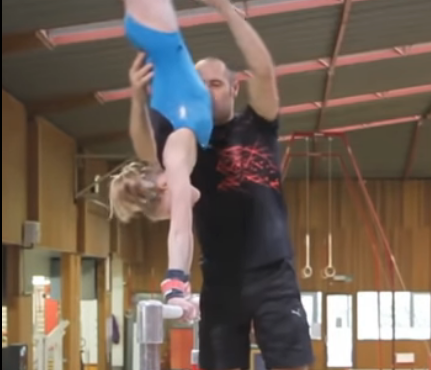
\includegraphics[width=\linewidth]{training1.png}
  \caption{Active Boundary}
\end{subfigure}%
\begin{subfigure}{.25\textwidth}
  \centering
  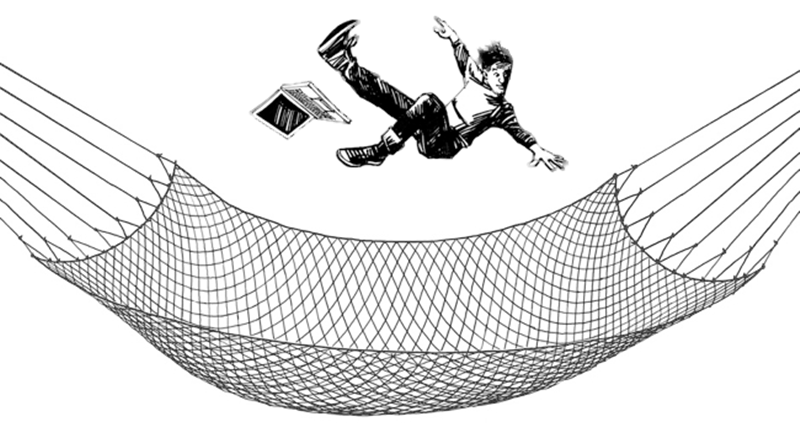
\includegraphics[width=\linewidth]{training2.png}
  \caption{Passive Boundary}
\end{subfigure}
\caption{Difference Between Active Boundary and Passive Boundary}
\label{fig:athelete}
\end{figure}

\section{Implement active Boundary in OpenAI Gym}
We implemented our active boundary experiments in OpenAI Gym\cite{Brockman2016OpenAIG} as a proof of concept. We are cognizant of the fact that eventually, things should apply to a real-world scenario. Therefore, we designed the active boundary in a manner such that it can be swiftly adapted to physical implementation. Agents are implemented with tensorforce\cite{tensorforce}. We sorted out the observation space and action space for each environment and recorded them in the code of each experiment.

As we suggested in the previous section when agents reach the critical state, "correct actions" would be applied by the active boundary to the agent, hence the name "active". Much like a coach would guide athletes through the most crucial step of the training. We also designed a penalty term associated with active boundary to discourage its use. If the agent act flawlessly at the critical state, no penalty would be applied. On the other hand, if the agent requires active boundary intervention, a penalty term would be registered. 

The positions and penalty terms are set in an ad hoc fashion in our experiments. At this point, we do not have an analytical frame that can guide us in making such decisions. We choose three positions for the boundary during each experiment and 4-6 penalty terms ranging from 0 upwards. The rule of thumb we used for the penalty is that the punishment score should be comparable to the reward.

Our experiments are conducted over the following environments: CartPole, with discrete action space; Inverted Pendulum, with continuous action space; Inverted Double Pendulum; Hopper; Walker2D. We did not implement our approach to more sophisticated environments such as HalfCheetah, Humanoid, and HumanroidStandup due to hardware constraints. Yet we feel that for the data we collected, our approach has shown conclusive results. The following are our experiment setup and results.

The dashed black lines are the training results of agents with normal training, which functions as the control group and the benchmark. The colored lines are the results of agents trained with varying penalty terms. The average evaluation scores of the agents are presented at the upper left corner of the graph.

\subsection{CartPole and Inveretd Pendulum}
CartPole's Observation Space is the vector: [Cart Position, Cart Velocity, Pole Angle, Pole Angular Velocity]. The discrete action space for cartpole is: [Push Cart to the left, Push cart to the right]. The continuous action space for Inverted Pendulum is an action ranging from -1 to 1, where -1 means the actuator moves the cart to the left with maximum power and 1 means the actuator moves the cart to the right with maximum power. The maximum episode step number for cartpole and inverted pendulum are 500 steps and 300 steps respectively. The terminal state for cartpole is angle of absolute value greater than 24 degrees. The terminal state for the inverted pendulum is an angle of absolute value greater than 0.2 radius. The reward for cartpole and inverted pendulum are both 1 for each step and 0 for the terminal step. 

The active boundary is implemented as a ring anchored on the cart, at the height of the middle of the pole. Touch sensors would be installed in order to detect contact between the pole and the ring. We propose three sets of rings each allows a maximum angle of 0.5, 0.7, and 0.9 of the terminal state angle in the cartpole environment and 0.1, 0.4, 0.5 radii in the inverted pendulum environment, as shown by Figure \ref{fig:cartpolePB}. 

\begin{figure}
     \centering
      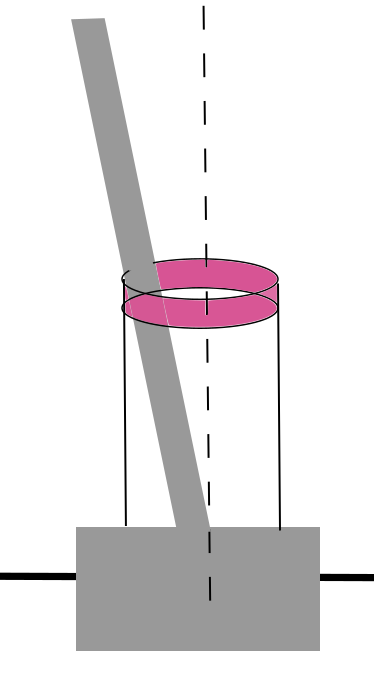
\includegraphics[width=0.1\textwidth]{cartpole1.png}
      \caption{CartPole/Inverted Pendulum active Boundary}
      \label{fig:cartpolePB}
\end{figure}
When contact between the pole and the active boundary is detected by the sensor, the cart would be pushed towards the appropriate direction depending on the sign of the angle. This step can be easily programmed by a microcontroller in physical implementation, and for implementation in simulation, it is just a matter of specifying a premeditated action. For detailed code, please refer to the code depository. Note that should the boundary is set without touch sensors and the corresponding actions, it would just be a passive boundary instead of an active one. 

A penalty term, which is chosen from vector [0,-5,-7,-10,-12,-15], would incur every time the pole contacts the active boundary. Our experiment result on cartpole are shown by Figure \ref{fig:CartPole}. The experiment result on inverted pendulum is shown by figure \ref{fig:InvertedPendulum}. As the data suggest, when the boundary is set too restrictively, it severely hinders the training. The best results is seen when the boundary is set at 10.8 degrees. After the agents are done training, we evaluate their performance in normal environments, the average evaluation scores are presented at the upper left part of the graphs. Our data suggest that during the evaluation, agents with accelerated training perform comparably to the agents with normal training.


\begin{figure}
    \centering
    \captionsetup[subfigure]{font=scriptsize,labelfont=scriptsize}
    \begin{subfigure}[b]{0.5\textwidth}
      \centering
      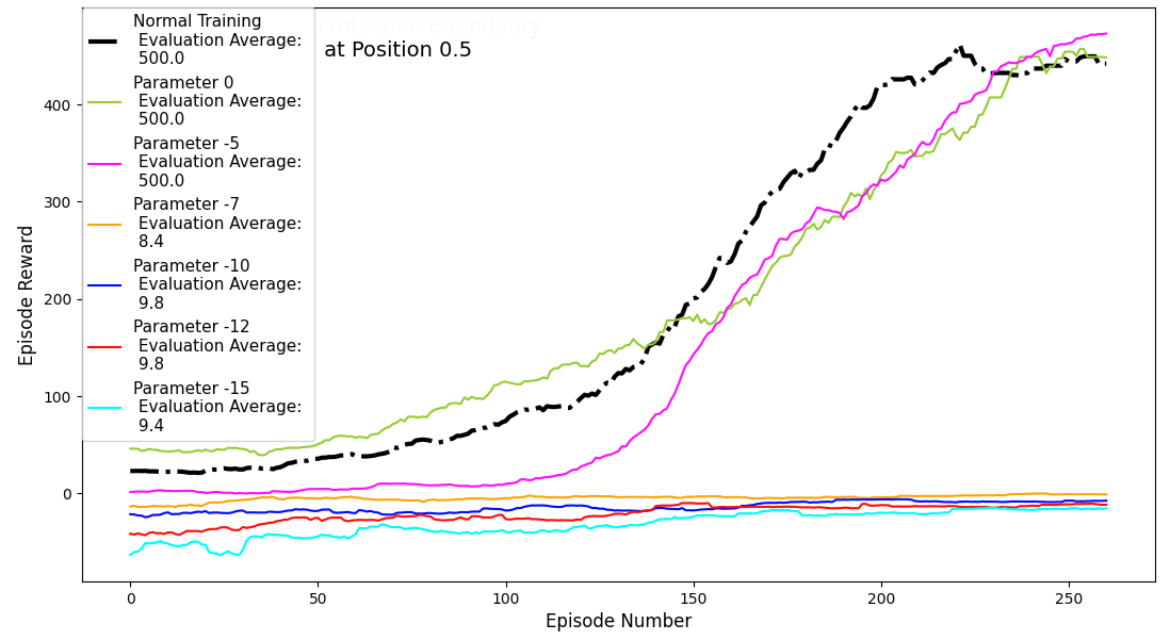
\includegraphics[width=\textwidth]{Cartpole_with_Boundary_at_0.5.png}
    \end{subfigure}
    \vspace*{0.0mm}
    \begin{subfigure}[b]{0.5\textwidth}
      \centering
      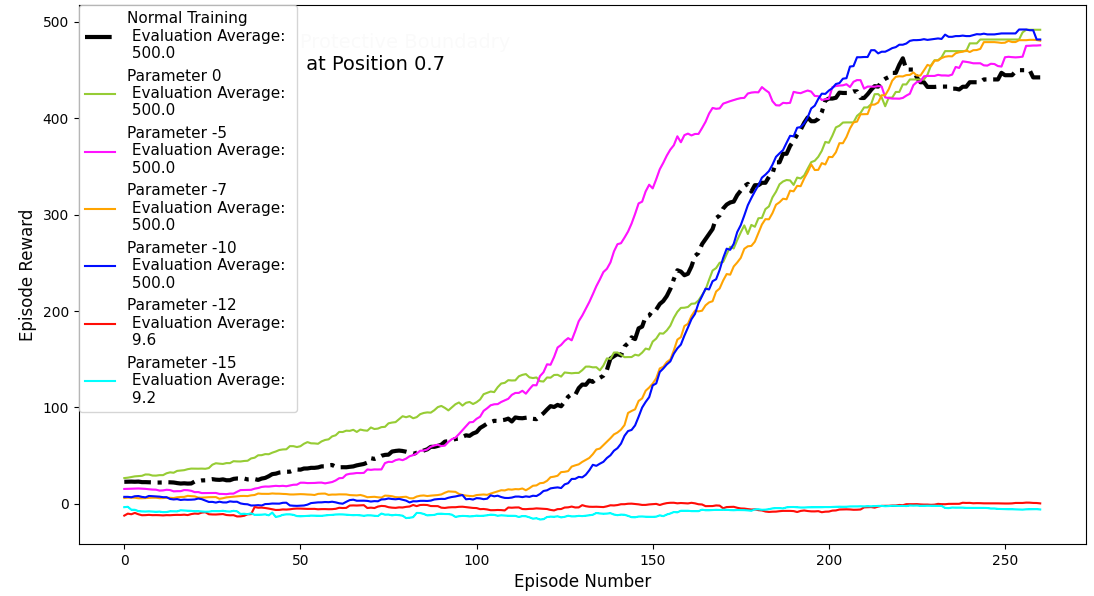
\includegraphics[width=\textwidth]{Cartpole_with_Boundary_at_0.7.png}
    \end{subfigure}
    \vspace*{0.0mm}
    \begin{subfigure}[b]{0.5\textwidth}
      \centering
      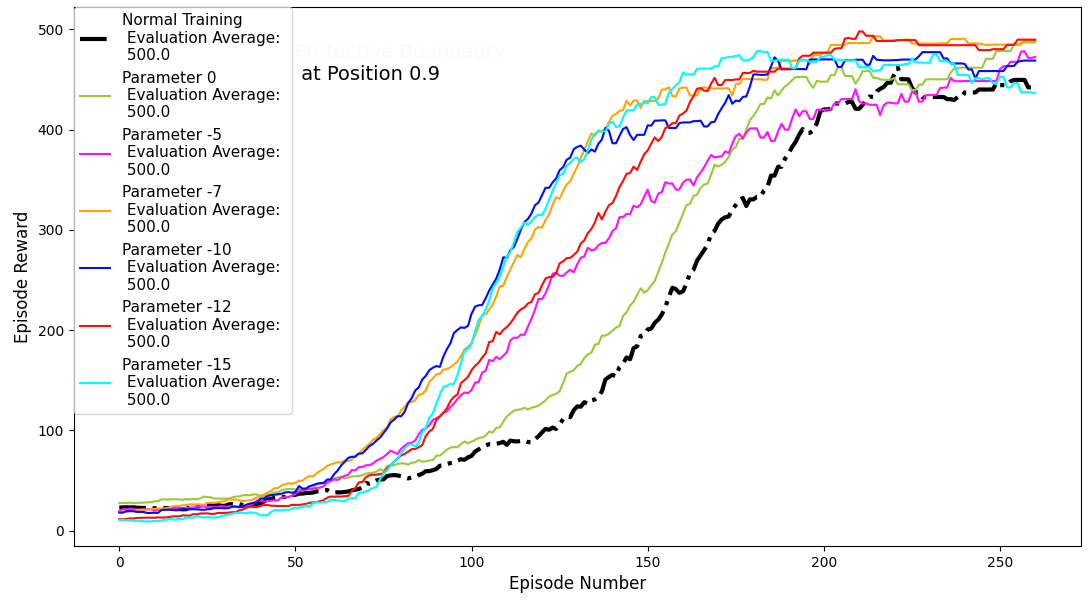
\includegraphics[width=\textwidth]{Cartpole_with_Boundary_at_0.9.png}
    \end{subfigure}
    \caption{CartPole Experiments}
    \label{fig:CartPole}
\end{figure}

\begin{figure}
    \centering
    \begin{subfigure}[b]{0.5\textwidth}
      \centering
      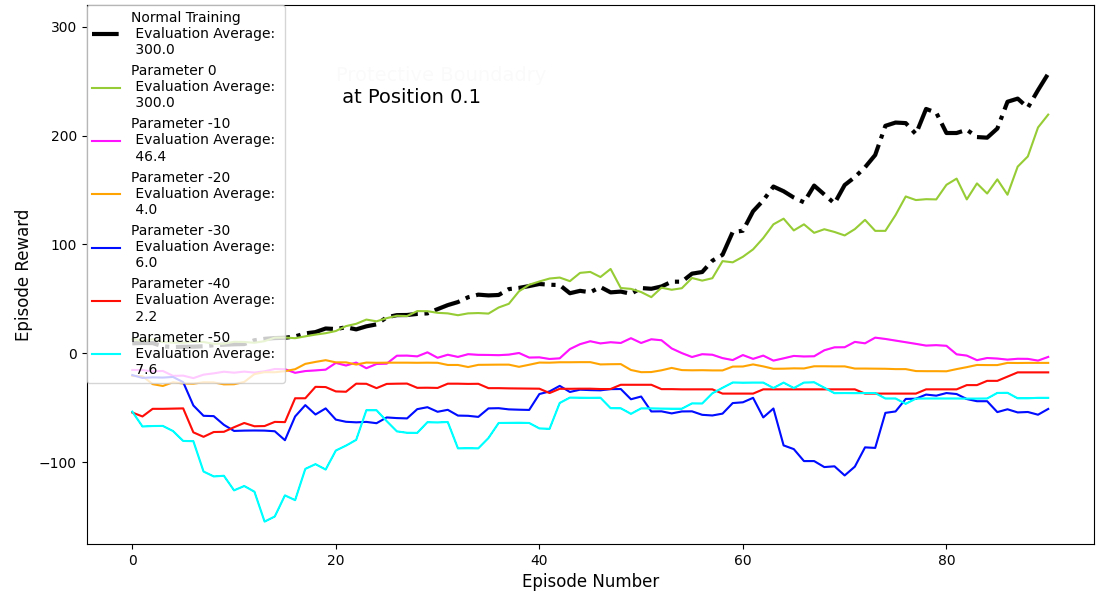
\includegraphics[width=\textwidth]{Inverted_Pendulum_with_Boundary_at_0.1.png}
    \end{subfigure}
    \vspace*{0.0mm}
    \begin{subfigure}[b]{0.5\textwidth}
      \centering
      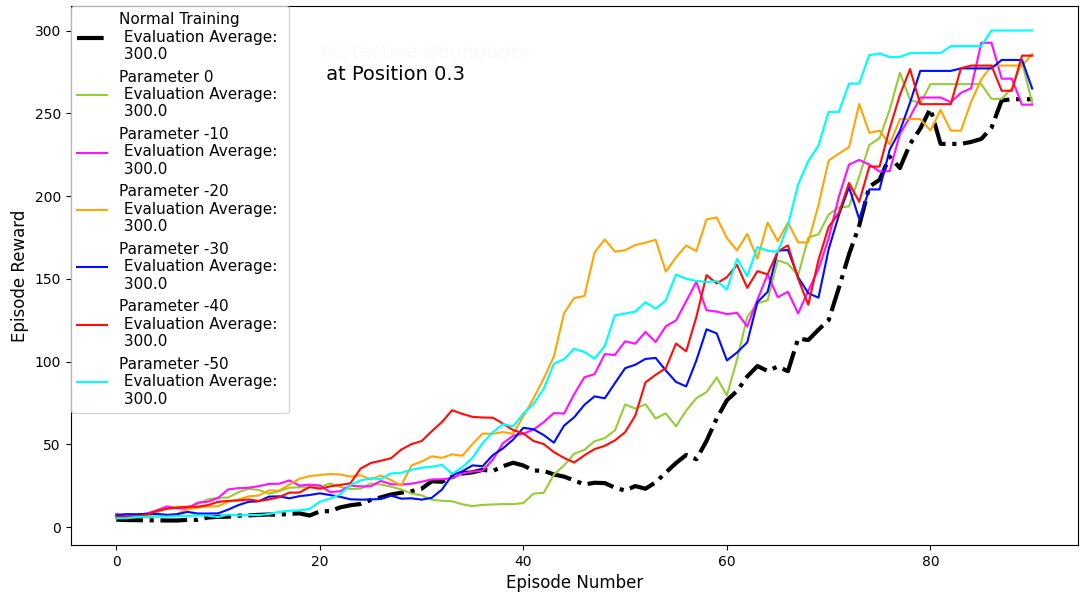
\includegraphics[width=\textwidth]{Inverted_Pendulum_with_Boundary_at_0.3.png}
    \end{subfigure}
    \vspace*{0.0mm}
    \begin{subfigure}[b]{0.5\textwidth}
      \centering
      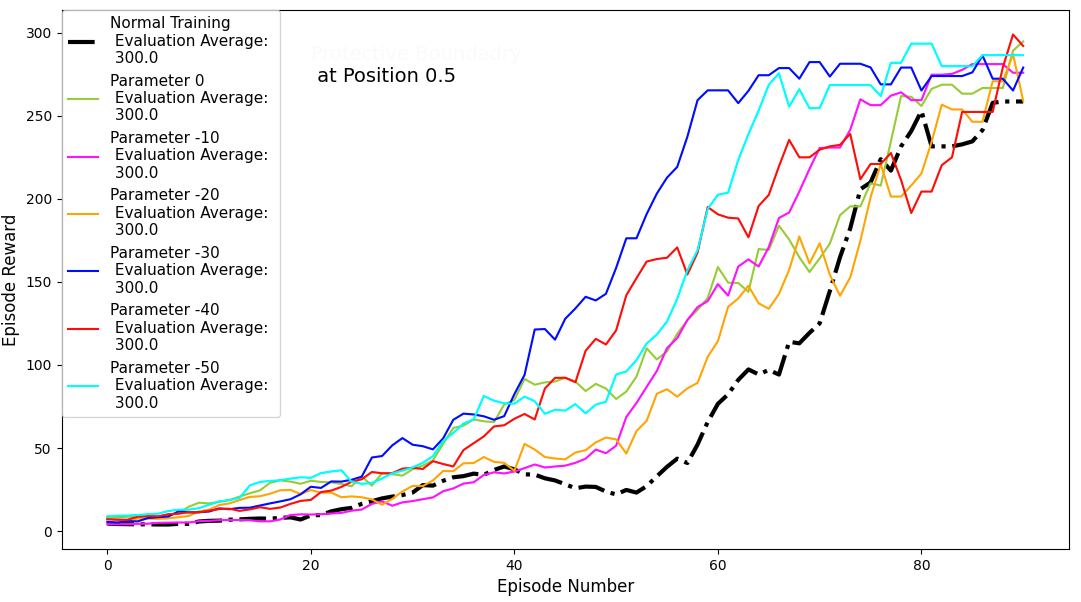
\includegraphics[width=\textwidth]{Inverted_Pendulum_with_Boundary_at_0.5.png}
    \end{subfigure}
    \caption{Inverted Pendulum Experiments}
    \label{fig:InvertedPendulum}
\end{figure}

\subsection{Inverted Double Pendulum}
The inveretd double pendulum has observation space of the following: [x position of the cart, sin($\theta_1$), sin($\theta_2$),cos($\theta_1$),cos($\theta_2$),velocity of x, angular velocity of $\theta_1$, angular velocity of $\theta_2$, constraint force on x, constraint force on $\theta_1$, constraint force on $\theta_2$]. $\theta_1$ and $\theta_2$ are the angles of the upper and lower pole perspectively.

The action space for Inverted Double Pendulum is an action ranging from -1 to 1, where -1 means the actuator moves the cart to the left with maximum power and 1 means the actuator moves the cart to the right with maximum power.

The Terminal state of double inveretd pendulum is when the y postion of the upper pole, which can not be observed by the agent, falls below 1.

We design the active boundary to be located at the same height as does the joint between the upper and the lower pole, as indicated by Figure \ref{fig:doublePB}. The boundary allows the joint to flex for 0.4, 0.5 and 0.6 radii respectively, each with the penalty parameters of a choice between 0,-3,-4,-5,-6,-7. When the joint extends to touch the active boundary, an action of -1 or 1 would be automatically applied to rectify the situation, depending on the sigh of the angles.

\begin{figure}
     \centering
      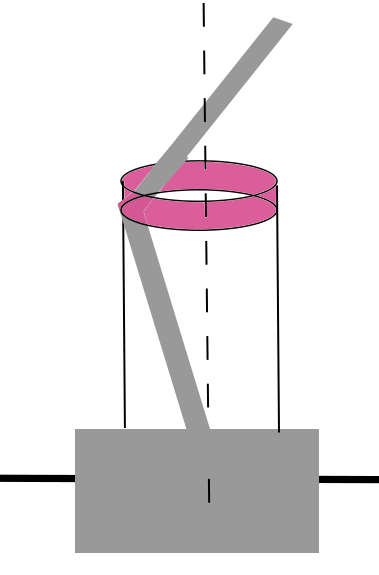
\includegraphics[width=0.1\textwidth]{cartpole2.png}
      \caption{Inveretd Double Pendulum active Boundary}
      \label{fig:doublePB}
\end{figure}

Our experiment result is shown by Figure \ref{fig:Double Pendulum}. The conclusion is similar to that of cartpole and inverted pendulum results. When the active boundary is set at 0.4 radii, it hinders learning rather than facilitate it. When the boundary is set at 0.5 radii with a penalty parameter of -7, we see the most drastic acceleration of agent training. However, when the boundary is set at 0.6 radii, it seems to have given the agent too much flexibility since the result suggests that the acceleration is not as profound compare to that of the boundary set at 0.5.

\begin{figure}
    \centering
    \begin{subfigure}[b]{0.5\textwidth}
      \centering
      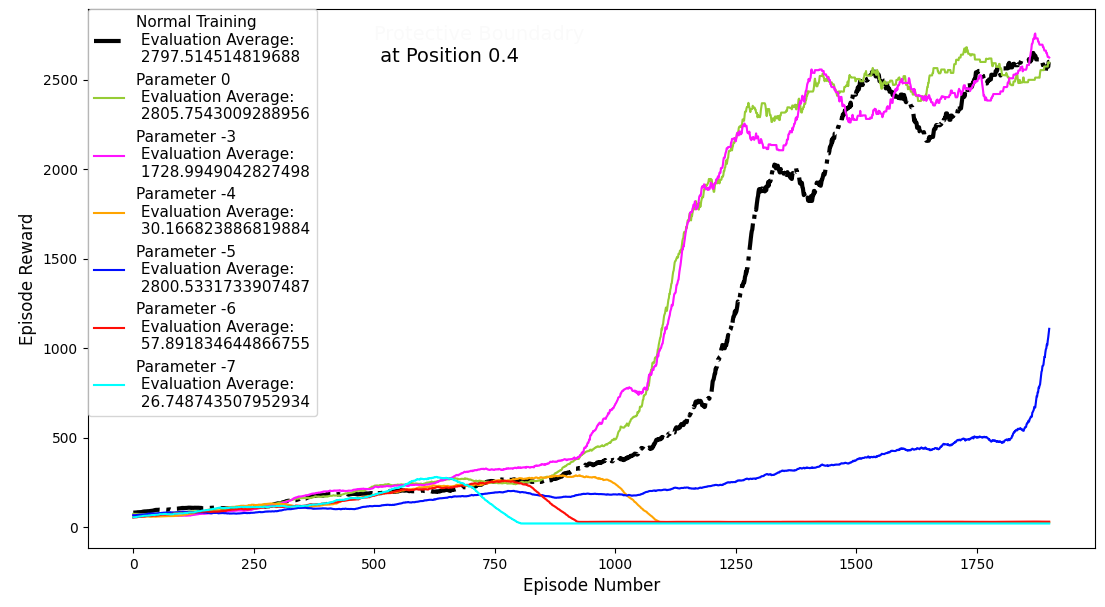
\includegraphics[width=\textwidth]{Double_Pendulum_with_Boundary_at_0.4.png}
    \end{subfigure}
    \vspace*{0.0mm}
    \begin{subfigure}[b]{0.5\textwidth}
      \centering
      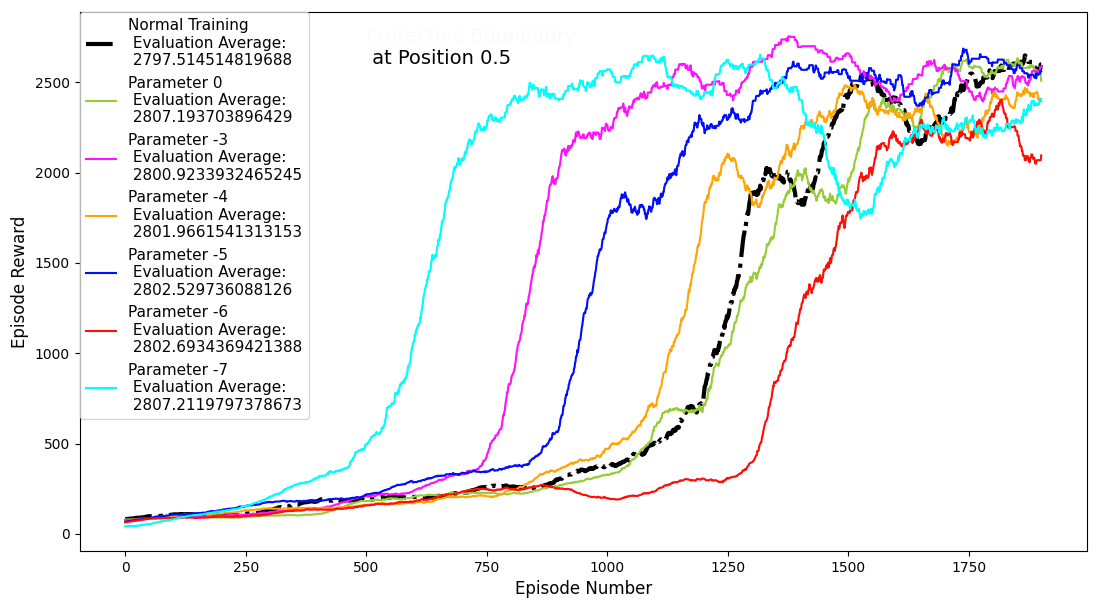
\includegraphics[width=\textwidth]{Double_Pendulum_with_Boundary_at_0.5.png}
    \end{subfigure}
    \vspace*{0.0mm}
    \begin{subfigure}[b]{0.5\textwidth}
      \centering
      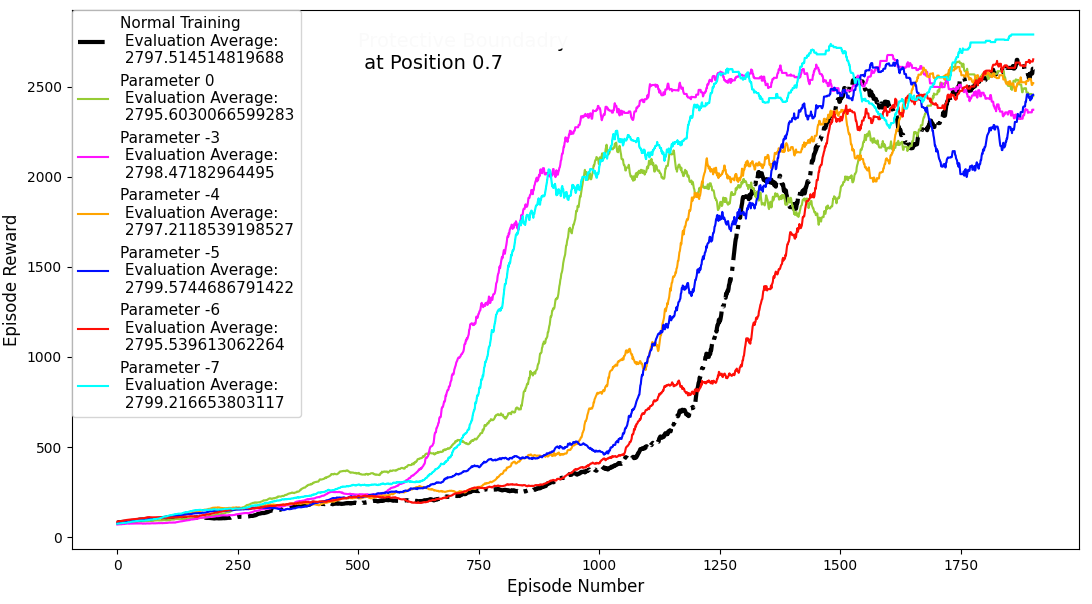
\includegraphics[width=\textwidth]{Double_Pendulum_with_Boundary_at_0.7.png}
    \end{subfigure}
    \caption{Inverted Double Pendulum Experiments}
    \label{fig:Double Pendulum}
\end{figure}


\subsection{Hopper}
The observation space of hopper is the following vector: [z position, y position, thigh joint angle, leg joint angle, foot joint angle, velocity at x-axis, velocity at z-axis, velocity at y-axis, angular velocity of thigh joint, angular velocity of leg joint, angular velocity of foot joint].

The action space of hopper are three continuous action choices for three actuators [thigh actuator, leg actuator, foot actuator]. The range of for actuators are -1, which means apply force towards the negative direction with maximum power, and 1 which means apply force towards the positive direction with maximum power.

The terminal states for hopper are when the absolute y position is greater than 0.2.

There are more than one ways to implement active boundary in hopper environment. Because we want things to be applicable in real-world scenarios, we chose the implementation with the easiest setup. In our experiment, the active boundary is defined with the y-position at 0.05, 0.1 and 0.15, each with the penalty parameters that is chosen from 0,-3,-5,-7,-10 as shown by Figure \ref{fig:hopperPB} When the agent touches the active boundary, we gently guide it slightly towards the center line, and the velocities terms are all set to zero. We seek to mimic how a coach would guide an athlete towards the desired trajectory during training. When the athlete is about to deviate off-course, the coach would take over and apply the appropriate force to slightly reset the trajectory. This can be implemented with an automatic harness in a physical experiment.

Our experiment result is shown by Figure \ref{fig:Hopper}. Similar to the conclusion drawn with previous data, when the active boundary is set too narrowly at 0.05 y position, it restricts the agent and almost completely halts the agent training. The best training acceleration is observed when the boundary is set at 0.15 y position.

\begin{figure}
     \centering
      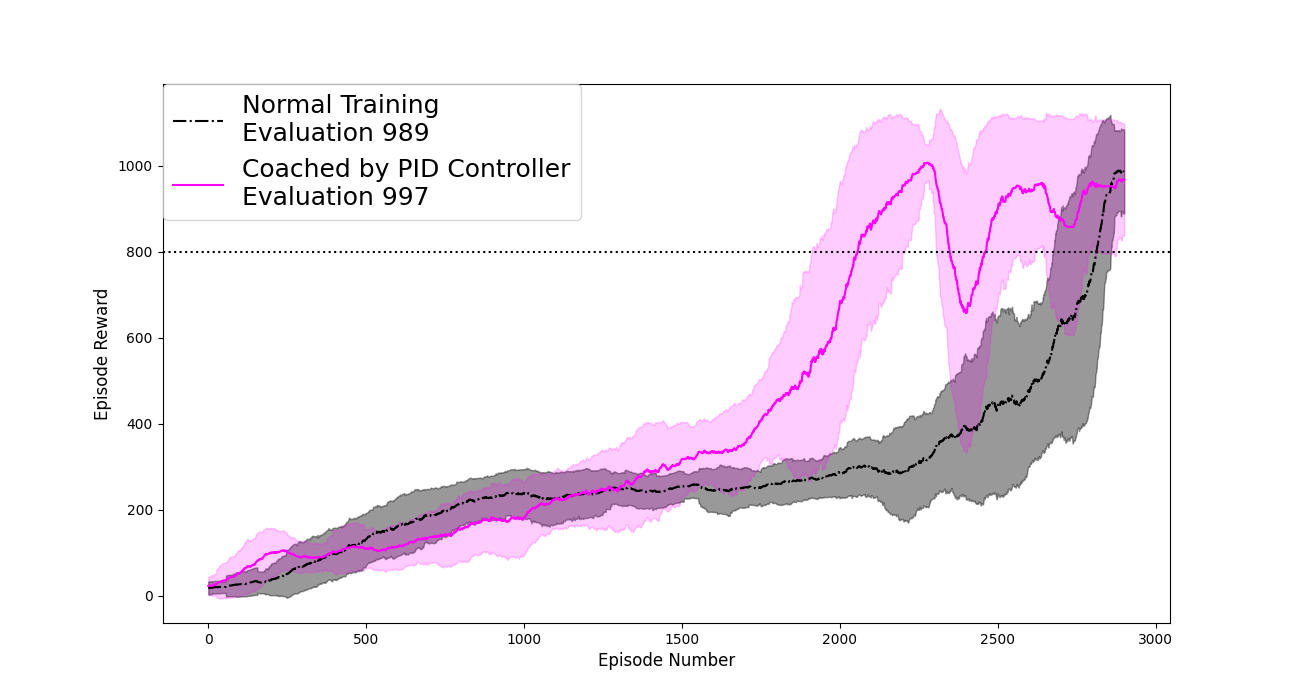
\includegraphics[width=0.2\textwidth]{hopper.png}
      \caption{Hopper active Boundary}
      \label{fig:hopperPB}
\end{figure}

\begin{figure}
    \centering
    \begin{subfigure}[b]{0.5\textwidth}
      \centering
      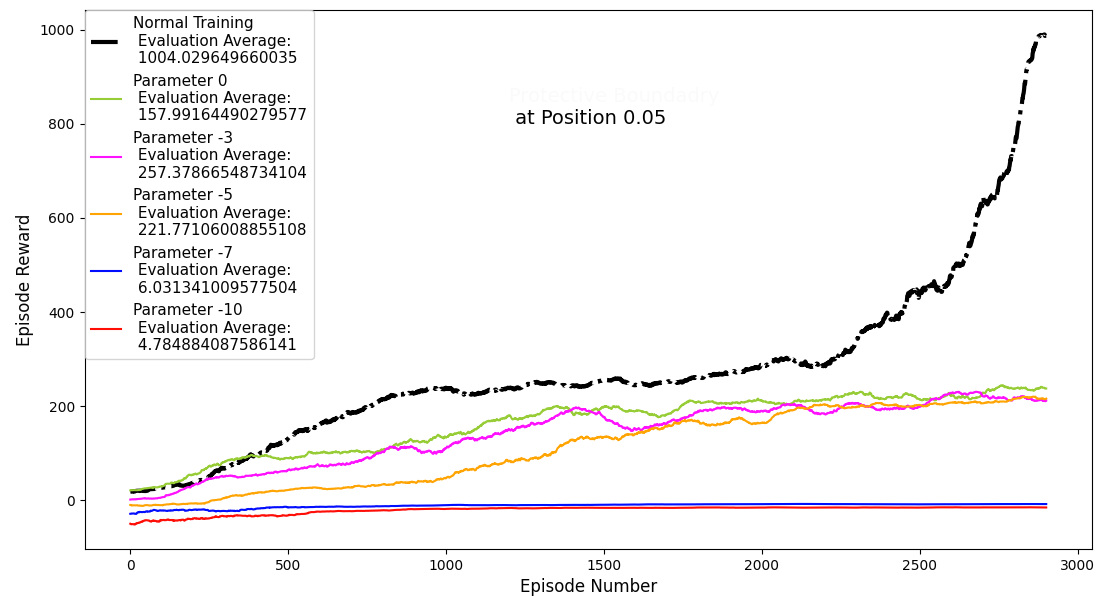
\includegraphics[width=\textwidth]{Hopper_with_Boundary_at_0.05.png}
    \end{subfigure}
    \vspace*{0.0mm}
    \begin{subfigure}[b]{0.5\textwidth}
      \centering
      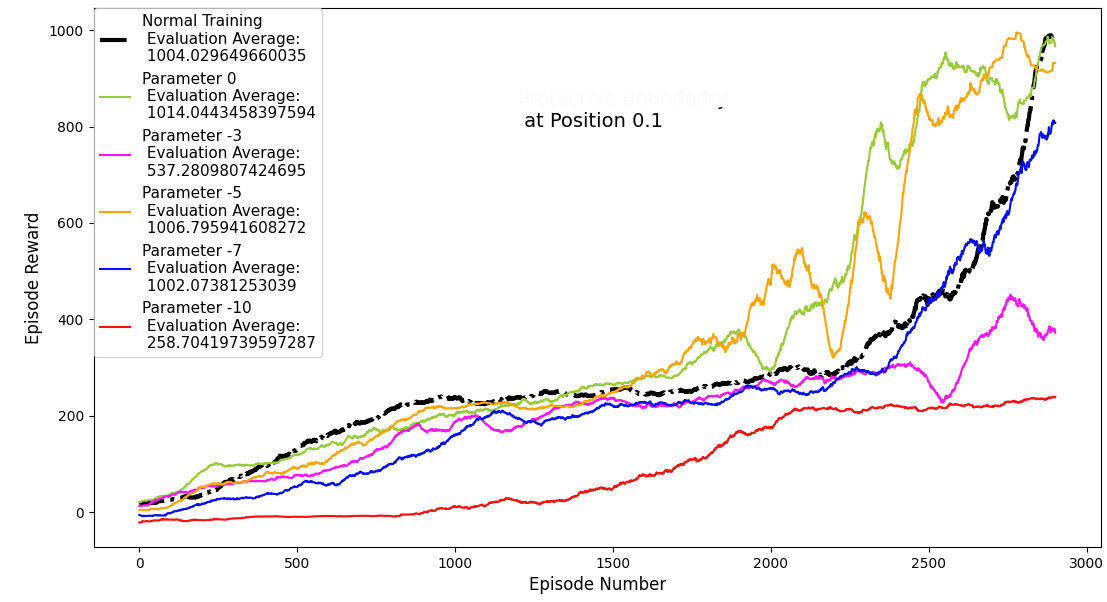
\includegraphics[width=\textwidth]{Hopper_with_Boundary_at_0.1.png}
    \end{subfigure}
    \vspace*{0.0mm}
    \begin{subfigure}[b]{0.5\textwidth}
      \centering
      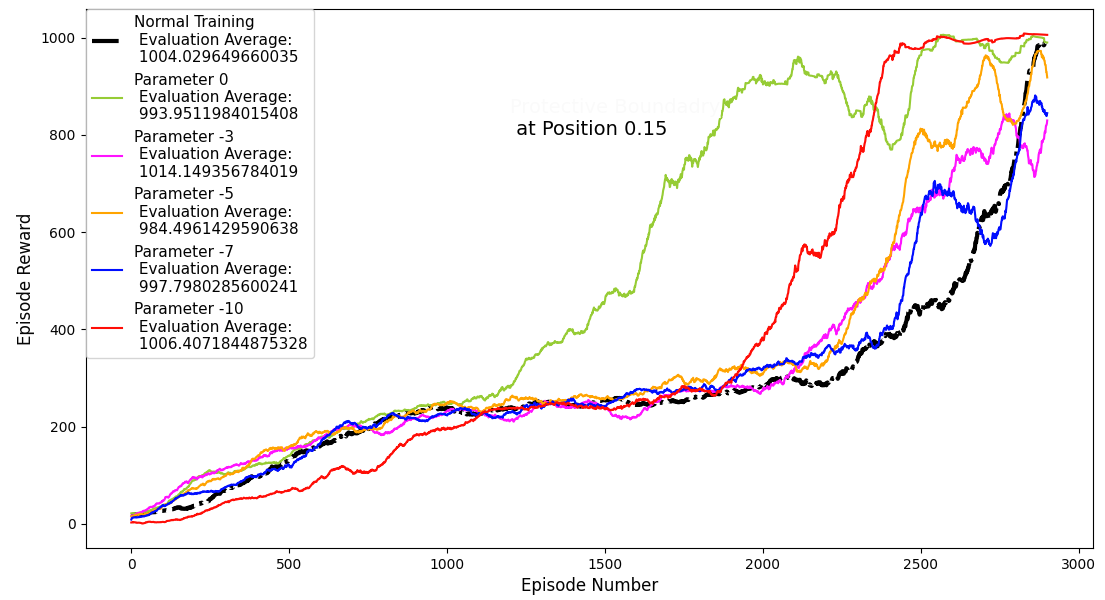
\includegraphics[width=\textwidth]{Hopper_with_Boundary_at_0.15.png}
    \end{subfigure}
    \caption{Hopper}
    \label{fig:Hopper}
\end{figure}


\subsection{Walker2d}
The walker environment's observation space is the following vector: [z position, y position, right thigh joint angle, right leg joint angle, right foot joint angle, left thigh joint angle, left leg joint angle, left foot joint angle, velocity along x axis, velocity along z axis, velocity along y axix, angular velocity for right thigh joint, angular velocity for right leg joint, angular velocity for right foot joint, angular velocity for left thigh joint, angular velocity for left leg joint, angular velocity for left foot joint]

There are 6 actuators for the right thigh joint, right leg joint, right foot joint and left thigh joint, left leg joint, left foot joint perspectively. The range for the motors is -1, which means apply force towards the negative direction with maximum power and 1, which means apply force towards the positive direction with maximum power.

The terminal states are when the z position falls below 0.8 or rise above 2 or the absolute value of y position is greater than 1.

The active boundary is set with the y position at 0.3, 0.7 and 0.9, each with the penalty parameters that is chosen from 0,-5,-10,-15,-20 as shown by Figure \ref{fig:walkerPB}. Similar to the active boundary for hopper, when the agent touches the active boundary in the walker environment, we gently guide it slightly towards the central line, and the velocities terms are all set to zero in the meantime.

Our experiment result is shown in Figure \ref{fig:Walker}. Yet again the experiment result suggests the same conclusion: when the boundary is positioned at 0.1, it acts as a barrier to training. When it is set at 0.7 positions, it could accelerate training with the appropriate penalty term.

\begin{figure}
     \centering
      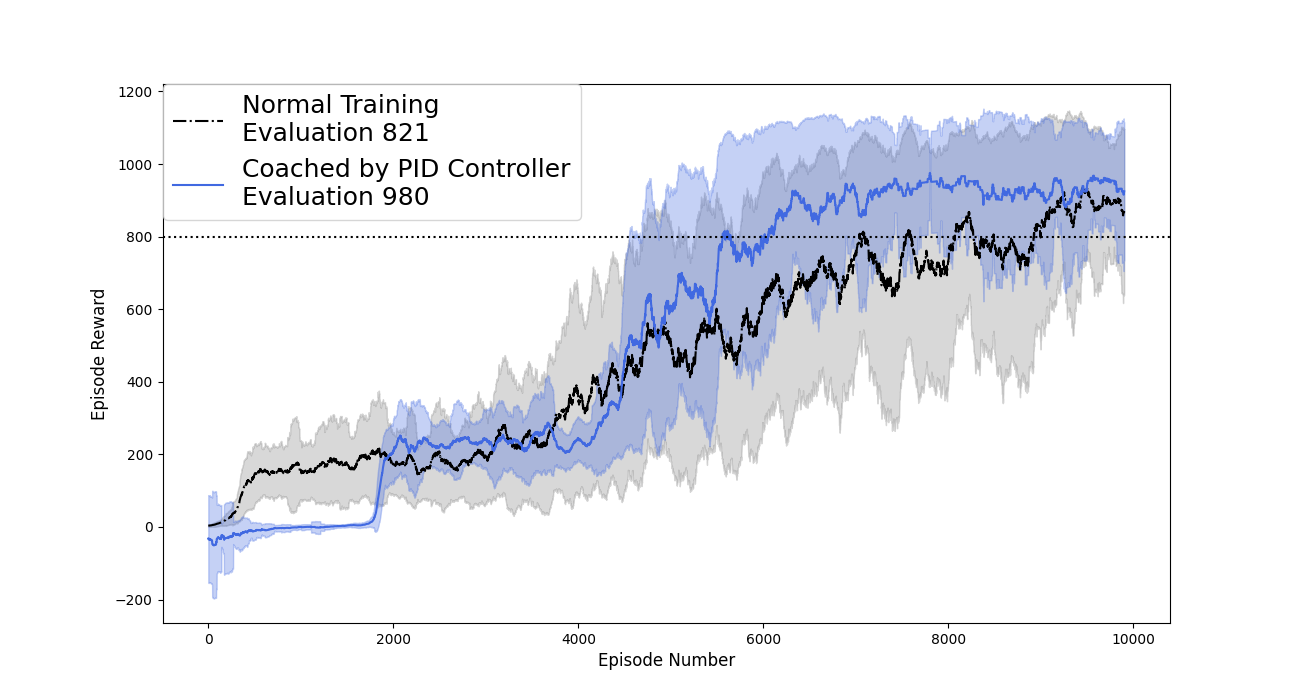
\includegraphics[width=0.2\textwidth]{walker.png}
      \caption{Walker2d active Boundary}
      \label{fig:walkerPB}
\end{figure}

\begin{figure}
    \centering
    \begin{subfigure}[b]{0.5\textwidth}
      \centering
      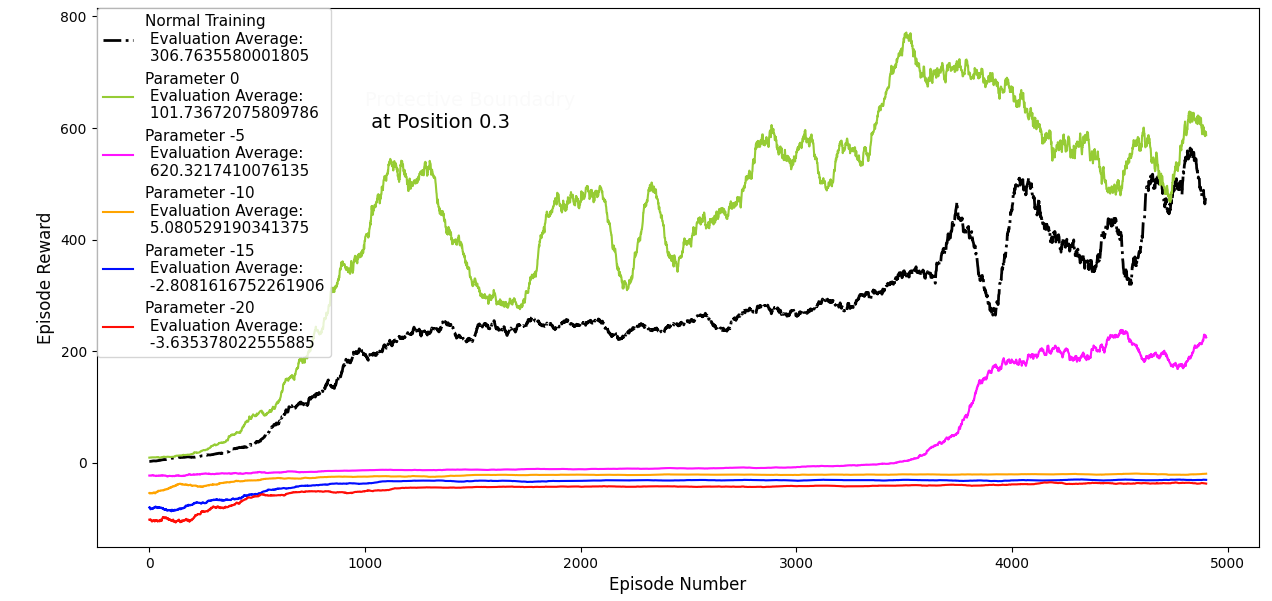
\includegraphics[width=\textwidth]{Walker_with_Boundary_at_0.3.png}
    \end{subfigure}
    \vspace*{0.0mm}
    \begin{subfigure}[b]{0.5\textwidth}
      \centering
      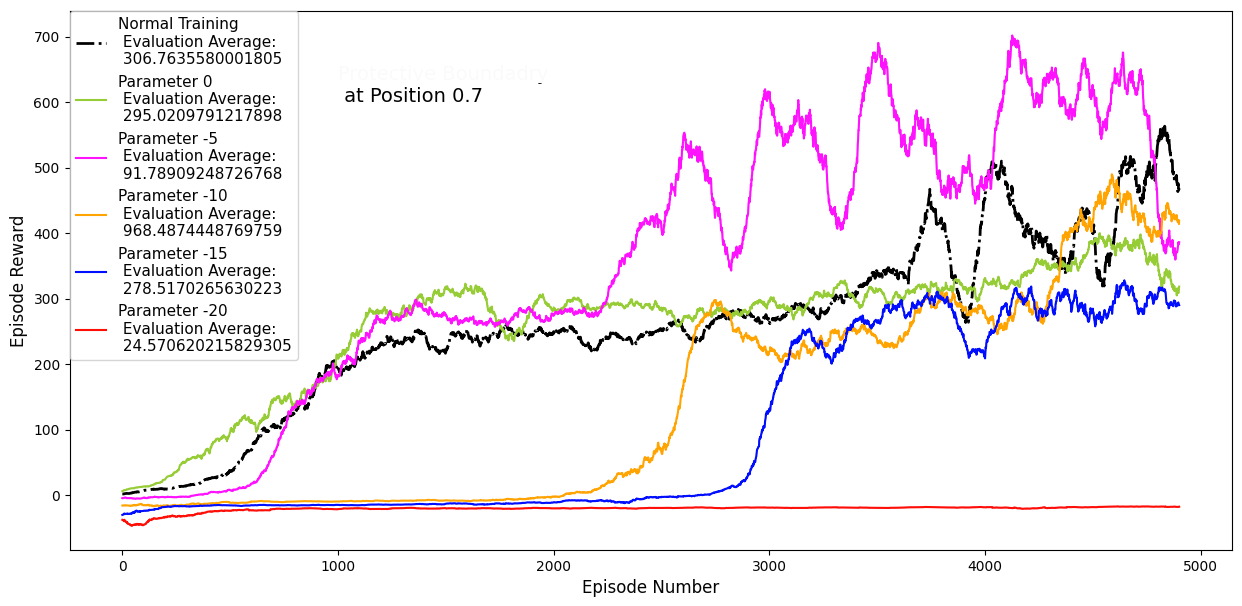
\includegraphics[width=\textwidth]{Walker_with_Boundary_at_0.7.png}
    \end{subfigure}
    \vspace*{0.0mm}
    \begin{subfigure}[b]{0.5\textwidth}
      \centering
      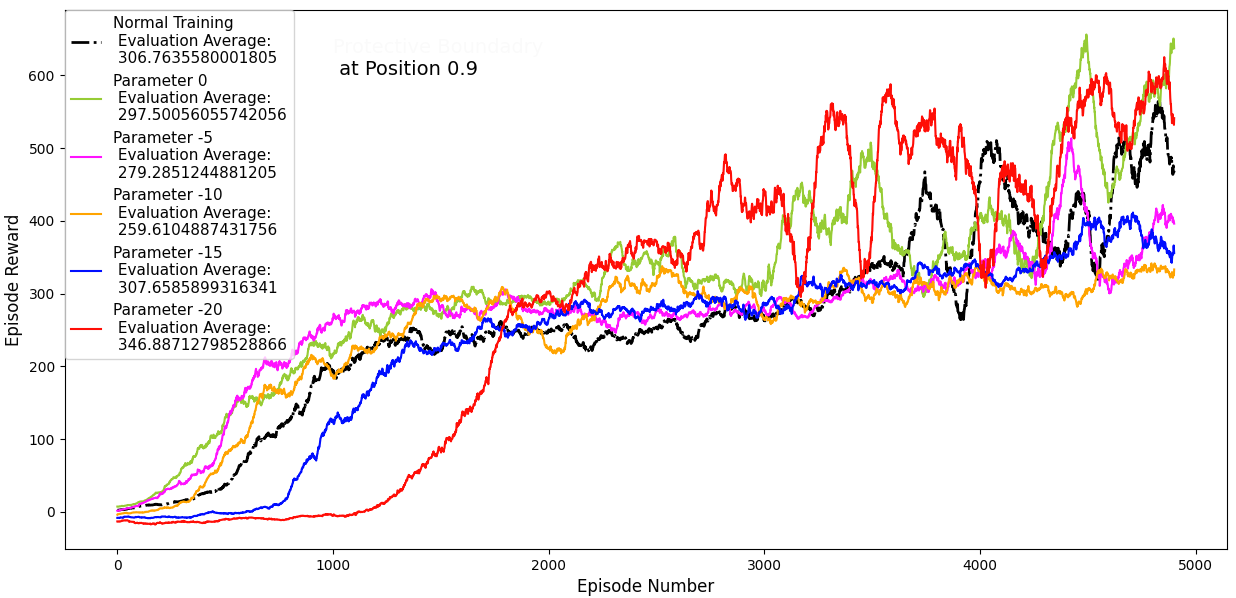
\includegraphics[width=\textwidth]{Walker_with_Boundary_at_0.9.png}
    \end{subfigure}
    \caption{Walker2D}
    \label{fig:Walker}
\end{figure}


\section{Conclution}

In this paper, we introduced the active boundary idea based on our observation of athletic training. Our proof of concept data suggests when the position and penalty associated with active boundary are set appropriately, accelerated learning can be achieved. Future research should focus on devising analytical tools that can systematically derive the best position and penalty for an active boundary.

Next step, we plan on extending the active boundary idea to the deep drone acrobat project \cite{Kaufmann2020DeepDA}. The training of drone acrobat is done in simulation and then transferred to a real-world drone controller. We think our active boundary method can greatly accelerate the training of drone acrobats. 

We believe our research opens door to a rich reservoir of potential researches along the direction of adapting proven human training techniques to RL environments. Human achieves superhuman feats not because of talent, but because of the meticulously engineered coaching tactics. Current researches in RL focus solely on the "athlete" side of the equation, i.e. how to build an efficient RL agent. But we feel "coach" is as important, if not more so.  For instance, the endgames training strategy was deployed to educate chess players. During the training phase, the agent should start the game middle way to amass experience with critical states, instead of wasting time on steps leading up to the critical position. Coaches also challenge athletes, pushing them to experience difficult situations. "Coach" could even be implemented by independent neural networks, in addition to the agent, and trained to "teach" better. All these should be investigated by future researches. 

\bibliographystyle{IEEEtran}
\bibliography{Bibliography}
%\printbibliography



\end{document}
